\documentclass[
	12pt,				% tamanho da fonte
	openright,			% capítulos começam em pág ímpar (insere página vazia caso preciso)
	oneside,			% para impressão apenas em um lado do papel
	a4paper,			% tamanho do papel.
	brazil				% o último idioma é o principal do documento
	]{abntex2}
\usepackage{etoolbox}
\usepackage{lmodern}			% Usa a fonte Latin Modern			
\usepackage[T1]{fontenc}		% Selecao de codigos de fonte.
\usepackage[utf8]{inputenc}		% Codificacao do documento (conversão automática dos acentos)
%\usepackage{lastpage}			% Usado pela Ficha catalográfica
\usepackage{indentfirst}		% Indenta o primeiro parágrafo de cada seção.
\setlength{\parindent}{1.5cm}   % Espaçamento de 1,5cm do parágrafo
\usepackage{color}				% Controle das cores
\usepackage{graphicx}			% Inclusão de gráficos
\usepackage{microtype} 			% para melhorias de justificação
\usepackage{lipsum}				% para geração de dummy text
\usepackage{abntex2cite}	% Citações padrão ABNT
\usepackage[table,xcdraw]{xcolor}% Cédula colorida em tabelas
%\usepackage{pdflscape}          % Rotaciona página
\usepackage{Capa}               % Capa e folha de rosto com modificações
\usepackage{float}              % Melhor posicionamento de figuras
\usepackage{gensymb}            % símbolo º
\usepackage[justification=justified,singlelinecheck=false]{caption}
%\usepackage{etoolbox}           % Configurações adicionais de macros
\usepackage{xparse}						
\usepackage{multirow}
\NewDocumentCommand\cc{+u{\cc}}{\ignorespaces}
\usepackage[justification=centering]{caption}
\usepackage{listings}

% --------------------
% Dados do Documento
% --------------------

\lstset{
  basicstyle=\ttfamily,
  keywordstyle=\color{blue},
  commentstyle=\color{green},
  stringstyle=\color{red},
  numbers=left,
  numberstyle=\tiny\color{gray},
  stepnumber=1,
  numbersep=5pt,
  showspaces=false,
  showstringspaces=false,
  tabsize=2,
  breaklines=true,
  breakatwhitespace=false
}
\titulo{Projeto de um circuito integrado de um pré-distorcedor digital baseado em polinômio de
memória}
\autor{Leonardo de Andrade Santos}
\data{\the\year}
\instituicao{Universidade Federal do Paraná}
\local{Curitiba}
\orientador[Orientadora:]{Sibilla Batista da Luz França}
\coorientador[Coorientador:]{Eduardo Gonçalves de Lima}
\preambulo{Trabalho de conclusão de curso do Curso de Graduação em Engenharia Elétrica da Universidade Federal do Paraná, como exigência parcial para obtenção do grau de Bacharel em Engenharia Elétrica.}


% ---------------------
% Configurações básicas
% --------------------

% informações do PDF
\makeatletter
\def\figsize{0.80\textwidth} % Define 80% da largura do texto
\hypersetup{
     	%pagebackref=true,
		pdftitle={\@title},
		pdfauthor={\@author},
    	pdfsubject={\imprimirpreambulo},
        pdfkeywords = {Desempenho Acadêmico}{Estatística Descritiva}{Evasão}{Vestibular},
		colorlinks=true,       		% false: boxed links; true: colored links
    	linkcolor=black,          	% color of internal links
    	citecolor=black,      	    % color of links to bibliography
    	filecolor=magenta,      	% color of file links
		urlcolor=black,
		bookmarksdepth=4
}
\makeatother

\graphicspath{{Figuras/}}

% -------------------
% Início do documento
% -------------------

\begin{document}

\frenchspacing % Retira espaço extra obsoleto entre as frases.

% ----------------------------------------------------------
% ELEMENTOS PRÉ-TEXTUAIS
% ----------------------------------------------------------

% ----
% Capa
% ----
\imprimircapa
% ---

% --------------
% Folha de rosto
% --------------
\imprimirfolhaderosto
% ---

%\begin{dedicatoria}  % Opcional
%\vspace*{\fill}
% Dedico este trabalho aos meus pais .....
%\vspace*{\fill}
%\end{dedicatoria}

% --------------
% Agradecimentos  % Opcional
% --------------

% \begin{agradecimentos}

% Inclua seus agradecimentos aqui. Há vários exemplos na internet.
% \end{agradecimentos}

% \begin{epigrafe} % Opcional
% \vspace*{\fill}
% \begin{flushright}
% \textit{"Democracia é oportunizar a todos o mesmo ponto de partida. \\
%          Quanto ao ponto de chegada, depende de cada um".\\
%          (Fernando Sabino)}
% \end{flushright}
% \end{epigrafe}

% ------
% Resumo
% ------
\newpage
\setlength{\absparsep}{18pt}   % ajusta o espaçamento dos parágrafos do resumo
\setlength{\abstitleskip}{1cm} % adiciona mais um cm após o 'titulo' do Resumo para ficar com 2cm,

% -------------------------------
% Lista de abreviaturas e siglas - Opcional
% -------------------------------

\begin{siglas}  %
 \item[DPD]  Pré-Distorcedor Digital
 \item[FPGA] Matriz de Portas Programáveis em Campo 
 \item[PA] Amplificador de Potência
 \item[RF] Rádio Frequência 
 \item[PARF] Amplificador de Potência de Rádio Frequência 
 \item[HDL] Linguagem de Descrição de software
 \item[VHSIC]  Circuito integrado de Velocidade Muito Elevada 
 \item[VHDL]  VHSIC Hardware Description Language
 \item[LUT]  Look Up Table
 \item[SOP]  Soma de Produtos 
 \item[LAB]  Logic Array Block 
 \item[ALM]  Adaptive Logic Module
 \item[LE]   Logic Element 
 \item[HEMT] transistor de efeito de campo de heterojunção
 \item[VSA] analisador de sinal vetorial  
 \item[NMSE] Erro Médio Quadrado Normalizado
\end{siglas}


\begin{resumo}

	A evolução dos sistemas de comunicação sem fio acarretou na implementação de diversas aplicações móveis e sem fio como desenvolvimento web, aplicação IoT, entre outros. Neste cenário, melhorar a eficiência energética se torna uma alternativa desejável tanto para os dispositivos móveis que buscam melhorar a autonomia das suas baterias, quanto para as estações de rádio base, que buscam reduzir sues desperdício em perdas de calor. No entanto, uma melhor eficiência energética implica em uma menor linearidade nos sistemas de amplificação de sinais, presentes nos sistemas transmissores de sinais de rádio. Isto é importante de ser ressaltado, pois a banda reservada para aplicações móveis é reduzida, de forma que para se alcançar maiores taxas de transmissão é necessário alternar estratégias de modulação tanto da fase, quanto da amplitude da onda portadora. E essas duas condições são conflitosas, já que a modulação AM é sensível a linearidade de forma que quanto mais linear um sistema ocorrem menos erros de transmissão. Sendo assim, uma alternativa para contornar esse obstáculo, que é implementar um sistema, eficiente energeticamente e linear é a implementação de um DPD em cascata com um PA. Portanto, o objetivo deste trabalho de conclusão de curso é o design de um circuito integrado dedicado de um DPD. Para atingir esse objetivo esse projeto foi divido em quatro etapas, o estudo e modelagem dos DPDs, modelagem do DPD em software, implementação do DPD em FPGA e finalmente o design do circuito integrado do DPD. Para a modelagem do DPD foi utilizada a métrica do NMSE, nela quanto menor o NMSE encontrado mais fiel e o modelo com a realidade. Sendo assim, na etapa de modelagem do PA alcançou-se um NMSE de -23.57 db. Em seguida, foi feita o levantamento do número de bits necessários para a realização desses cálculos de forma a minimizar o NMSE, para isso foi verificado que com apenas 8 bits de resolução do sinal já foi possível alcançar um NMSE próximo do valor alcançado em virgula flutuante. Portanto, ainda restam as etapas de implementação do DPD em FPGA e o design do circuito integrado. 

\textbf{Palavras-chave}: VHDL, FPGA, DPD 

	.
	\end{resumo}

	
\listoffigures*
\cleardoublepage
% -------
% Sumario
% -------
\pdfbookmark[0]{\contentsname}{toc}
\tableofcontents*
\cleardoublepage
% ---

\makepagestyle{abntheadings}
\makeevenhead{abntheadings}{\ABNTEXfontereduzida\thepage}{}{}
\makeoddhead{abntheadings}{}{}{\ABNTEXfontereduzida\thepage}
\makeheadrule{abntheadings}{\textwidth}{0in}

% ----------------------------------------------------------
% ELEMENTOS TEXTUAIS
% ----------------------------------------------------------

\textual

\setcounter{page}{1}

\chapter{Introdução} 
\label{chap:introducao}
A evolução dos sistemas de comunicação móveis, impulsionada pela crescente demanda por comunicações mais rápidas e eficientes, tem levado à implementação de uma variedade de serviços, incluindo aplicações multimídia, desenvolvimento web e aplicações IoT \cite{John2016}. No entanto, essa evolução também trouxe desafios significativos, como a necessidade de melhorar a eficiência energética, tanto para dispositivos móveis, visando aumentar a autonomia da bateria, quanto para estações de rádio base, visando reduzir o consumo de energia devido às perdas de calor. Para atender a essas demandas, estratégias de modulação que alteram tanto a fase quanto a amplitude de ondas portadoras em radiofrequência se tornaram essenciais \cite{Kenington2000}. Além disso, a modulação na amplitude requer linearidade na transmissão para evitar erros e interferências na comunicação entre usuários vizinhos \cite{Cripps2006}. Essa complexa tarefa recai sobre o projetista do PARF (Amplificador de Potência de Rádio Frequência), que enfrenta o desafio de desenvolver um hardware eficiente em termos energéticos e linear ao mesmo tempo, uma vez que esses dois objetivos podem entrar em conflito \cite{Chavez2018}. Uma solução para contornar esse desafio é a implementação de um pré-distorcedor de Sinais Digital em Banda Base, que visa compensar a distorção causada pelo PARF \cite{Cripps2006}. O DPD (Pre-distorcedor Digital) é conectado em cascata ao PARF e requer um modelo de alta precisão e baixa complexidade computacional para representar as características de transferência direta e inversa do PARF. Existem duas abordagens para modelar o PARF: modelos físicos, que são detalhadas e computacionalmente complexos, e modelos empíricos, que se baseiam em medições de entrada e saída do PARF, com menor complexidade computacional, mas com uma possível diminuição da precisão. Devido às exigências rigorosas de frequência de operação, a paralelização das operações torna-se essencial, e as FPGAs (Matriz de Portas Programáveis em Campo) emergem como uma alternativa viável para a implementação de circuitos pré-distorcedores \cite{Pedroni2010}. As FPGAs são dispositivos lógicos programáveis que permitem a reconfiguração física de componentes de eletrônica digital, acelerando processos e suportando operações paralelas e sequenciais. Neste contexto esse projeto foi planejado com os seguintes objetivos geral e específicos:

\subsection{Objetivo Geral}
Construção e validação de um código em linguagem de descrição de hardware capaz de processar em tempo real as características de transferência de um amplificador. O código deve ser capaz de reproduzir não linearidades e efeitos de memória. Além disso, o código deve ocupar a quantidade mínima de recursos lógicos do circuito digital que irá sintetizá-lo, buscando reduzir o consumo de energia.


\subsection{Objetivos Específicos}
Para alcançar o objetivo geral, este trabalho foi desenvolvido com base nos seguintes objetivos específicos:

\begin{enumerate}
    \item Modelar com precisão o PA em software;
    \item Modelar o DPD em software a partir da modelagem do PA;
    \item Implementar o DPD em hardware utilizando uma HDL;
\end{enumerate}



\chapter{Revisão de Literatura} 
\label{chap:revi}
A evolução dos sistemas de comunicações sem fio, fomentou a implementação de diversas aplicações móveis. Neste contexto, melhorar a eficiência energética desses sistemas se torna uma característica desejável, tanto para os dispositivos móveis que buscam melhorar a autonomia das baterias quando para os sistemas de comunicação radio base que, tendem a perder energia em forma de calor.  
Sendo assim, o sistema de comunicação pode ser dividido em 3 sub-sistemas principais: Meio transmissor, Receptor e o Transmissor, conforme argumentado por \cite{Schuartz2017}.
No entanto, este trabalho foca exclusivamente no sistema transmissor, ilustrado pela figura \ref{fig:sistemadetrasmissao}, em que observa-se diversos componentes que compõem o transmissor de sinal entre esses elementos o amplificador de potência é o componente de maior demanda energética, por se tratar do componente que converte a energia da fonte em energia irradiada pela antena de transmissão. Portanto, a eficiência do sistema de transmissão depende diretamente do desempenho do transmissor. 

% // TODO Refazer figura
\begin{figure}[!ht!]
    \centering
    \captionsetup{justification=centering}
    \caption*{Fonte: \cite{Schuartz2017}}
    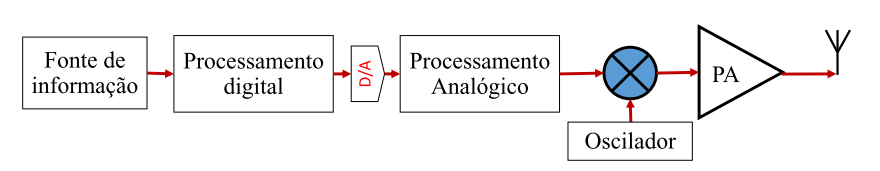
\includegraphics[width=0.5\textwidth]{sistematrasmissorpng.png}
    \caption{Sistema de transmissão simplificado}
    \label{fig:sistemadetrasmissao}
\end{figure}

Considerando também que a largura de banda reservada para sistemas de comunicação sem fio é reduzida, torna-se desejável que ela seja utilizada da maneira mais eficiente o possível. Diante desse cenário, segundo \cite{Kenington2000}, só é possível alcançar as maiores taxas utilizando estratégias de modulações, que alterem tanto a fase quanto a amplitude de uma onda portadora em rádio frequência. Ainda segundo \cite{Kenington2000}, a modulação na amplitude, exige linearidade na transmissão afim de evitar erros e interferência na comunicação entre os usuários vizinhos. Ante esse panorama, o projetista do PARF se depara com esse desafio, que é desenvolver um hardware eficiente energeticamente e com uma boa linearidade, o que é um compromisso é conflitante, conforme descrito por \cite{Cripps2006}. Esse comportamento se deve, ao fato que um PARF atua de forma eficiente, ou seja, com baixo consumo de energia, na área próxima à de saturação, que é a região em que opera em regimes não lineares, conforme ilustrado pela figura \ref{fig:saidaparf}.



\begin{figure}[ht!]
    \centering
    \captionsetup{justification=centering}
    \caption*{Fonte: \cite{Chavez2018}}
    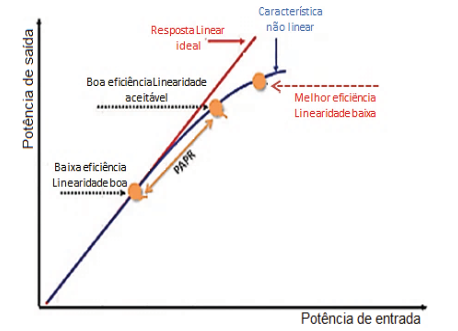
\includegraphics[width=0.5\textwidth]{curvasaidaparf.png}
    \caption{Curva de saída do amplificador}
    \label{fig:saidaparf}
\end{figure}

A fim de contornar esse obstáculo foi adicionado a cadeia de transmissão um método de equalização de sinais, conforme argumentado por \cite{Kenington2000}. Um exemplo de técnica de linearização de sinais é a implementação de um pré-distorcedor de sinais digitais em banda base, o qual apresenta um melhor custo-benefício \cite{Kenington2000}. Essa técnica consiste em distorcer o sinal de entrada utilizando técnicas de processamento digital, antes que esse module uma portadora, de forma compensativa à distorção causada pelo PARF. De maneira sucinta, o DPD é conectado em cascata ao PARF e é projetado de forma que apresenta a função transferência inversa ao PARF. Para isso, é necessário um modelo de alta precisão e baixa complexidade computacional, capaz de representar as características de transferência direta e inversa de um PARF. Isso significa modelar o seu comportamento real utilizando um software.  A figura \ref{fig:cascatadpd} ilustra o processo do um pré-distorcedor digital.

\begin{figure}[h!]
    \centering
    \captionsetup{justification=centering}
    \caption*{Fonte: \cite{Chavez2018}}
    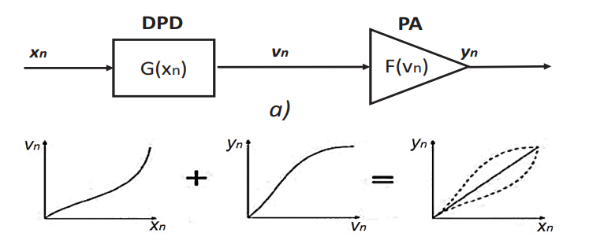
\includegraphics[width=0.5\textwidth]{DPDcascata.png}
    \caption{ilustração do pré-distorcedor em cascata}
    \label{fig:cascatadpd}
\end{figure}

Segundo \cite{John2016}, existem duas técnicas utilizadas para fazer essa modelagem. Uma consiste na descrição detalhada do PARF, que implica em uma maior complexibilidade computacional, esses modelos são conhecidos como modelos físicos. A outra abordagem é conhecida como modelo empírico, este modelo consiste em coletadas amostradas na entrada e na saída do PARF em domínio temporal, e através destes dados simulam um modelo matemático do sistema. Uma das vantagens desse método é que ele não exige conhecimento prévio da estrutura do PARF e possui baixa complexidade computacional e mesmo se todos os parâmetros fossem conhecidos o equacionamento completo do circuito, uma função inversa poderia ser encontrada, possivelmente muito mais complexa que séries de Volterra. No entanto, sua precisão pode ser ligeiramente afetada pelo modelo adotado. 
Sendo assim, como a proposta do projeto é a implementação de um DPD em hardware, se faz necessário que o circuito apresente a menor complexidade possível,  torna-se mais viável fazer a implementação utilizando modelagem matemática. 

\section{Modelagens Matemáticas}

\subsection*{Séries de Volterra}
Segundo \cite{Gonçalves2009} série de Volterra pode ser vista como uma extensão multidimensional da série de Taylor para sistemas dinâmicos. A modelagem começa com a representação do sistema através de uma série infinita de integrais convolucionais, em que cada termo da série corresponde a uma ordem de não linearidade e memória.

A saída \( y(t) \) de um sistema pode ser expressa pela equação \ref{eq:Volterra}: \begin{equation}
    y(t) = h_0 + \sum_{n=1}^{\infty} \int_{-\infty}^{\infty} \cdots \int_{-\infty}^{\infty} h_n(\tau_1, \tau_2, \ldots, \tau_n) \prod_{i=1}^{n} x(t - \tau_i) \, d\tau_i
    \label{eq:Volterra}
\end{equation} onde \( h_n \) são os núcleos de Volterra, que caracterizam a resposta do sistema para a \( n \)-ésima ordem de não linearidade e \( x(t) \) é a entrada do sistema.

Os núcleos de Volterra \( h_n \) são funções de várias variáveis que capturam a dinâmica do sistema em diferentes ordens. Para a maioria das aplicações práticas, a série é truncada para incluir apenas um número finito de termos, já que a identificação de todos os núcleos de uma série infinita é impraticável.

\subsection*{Polinômio de memória}\label{sub:polimem}

Um modelo simples, utilizado na modelagem comportamental simplifificada das séries de Volterra considerando apenas componentes unidimensionais\footnote{Cada termo do somatório é composto por amostras no mesmo instante, por exemplo: $x(n)|x(n)|,x(n - 1)|x(n - 1)|$; termos bidimensionais são compostos por amostras em instantes de tempos distintos, como por exemplo: $x(n)|x(n - 1)|$} é o MP, que é um modelo compacto, de baixo custo computacional e linear em seus parâmetros. O MP gera baixo erro quando aplicado à PAs que apresentam pouco efeito de memória. O DPD e pós distorsor apresentam uma característica de transferência inversa a do PA \cite{Schuartz2017}, portanto o mesmo modelo pode ser utilizado. A equação \ref{eq:mp} apresenta o MP conforme apresenta \cite{Schuartz2017}: 

\begin{equation}
    y(n) = \sum_{p=1}^{P} \sum_{m=0}^{M} h_{p,m} x(n - m) \left| x(n - m) \right|^{p-1}
    \label{eq:mp}
\end{equation}

Como a proposta do trabalho é a implementação em hardware desse modelo, torna-se necessário paralelizar operações aritméticas de forma a alcançar uma taxa de operação que satisfaça a norma regulamentadora. Nesse contexto, as FPGAs apresentam-se como uma alternativa viável para a implementação de circuitos pré-distorcedores 

\section{FPGAs}

Como descrito em \cite{Pedroni2010}, FPGAs são uma classe de dispositivos lógicos programáveis que permitem a reconfiguração física de seus componentes de eletrônica digital por meio de uma linguagem de descrição de hardware. Basicamente, as FPGAs consistem em um conjunto de subcircuitos digitais interconectados, capazes de realizar diversas funções comuns enquanto oferecem um alto nível de flexibilidade. Devido a essas características, FPGAs podem ser utilizadas para aplicações como processamento de imagem em tempo real e aprendizado de máquina.

FPGAs têm a capacidade de sintetizar arquiteturas complexas de eletrônica digital, resultando em um funcionamento altamente paralelizado que permite um processamento rápido com várias portas de entrada e saída. Além disso, elas também suportam o desenvolvimento de códigos sequenciais.

A estrutura interna de uma FPGA é composta fundamentalmente por blocos lógicos interligados, organizados em uma matriz. Cada bloco é formado por diversos sub-blocos, que por sua vez contêm os componentes mais básicos da hierarquia. FPGAs da Intel e da Xilinx possuem nomenclaturas e organizações diferentes para esses blocos e sub-blocos. Isso é ilustrado na Figura \ref{fig:Stratix} e na Figura \ref{fig:Ultrascale}, que mostram as FPGAs Intel Stratix X e Xilinx Ultrascale+, respectivamente. Embora as arquiteturas sejam fundamentalmente semelhantes, com a disposição em matriz dos blocos e funcionalidades dos componentes fundamentais sendo universais, os blocos lógicos são denominados LAB nas FPGAs da Intel e CLB nas FPGAs da Xilinx. Os sub-blocos são chamados de ALM ou LE, dependendo da FPGA da Intel, e de Slices nas FPGAs da Xilinx.

\begin{figure}[h!]
    \centering
    \captionsetup{justification=centering}
    \caption*{Fonte: \cite{Pedroni2010}}
    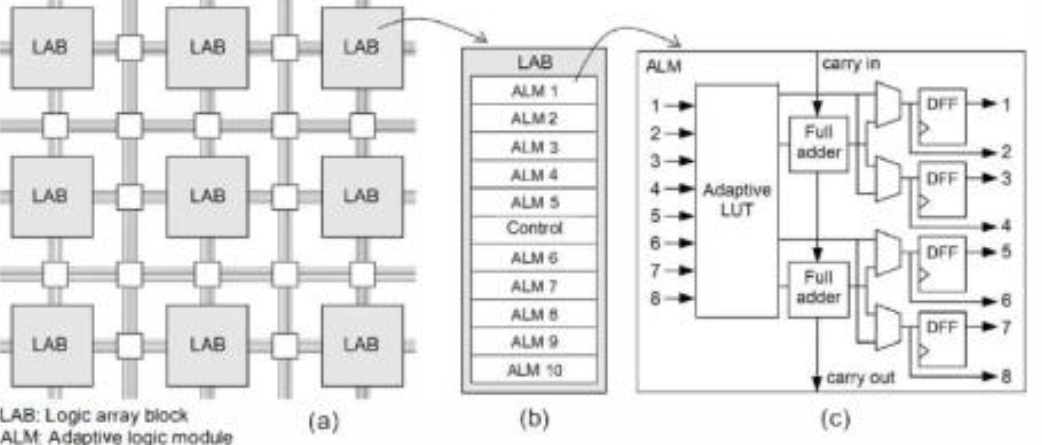
\includegraphics[width=0.75\textwidth]{FPGA Stratix X da Intel.png}
    \caption{Estrutura Interna da FPGA Stratix X da Intel}
    \label{fig:Stratix}
\end{figure}

\begin{figure}[h!]
    \centering
    \captionsetup{justification=centering}
    \caption*{Fonte: \cite{Pedroni2010}}
    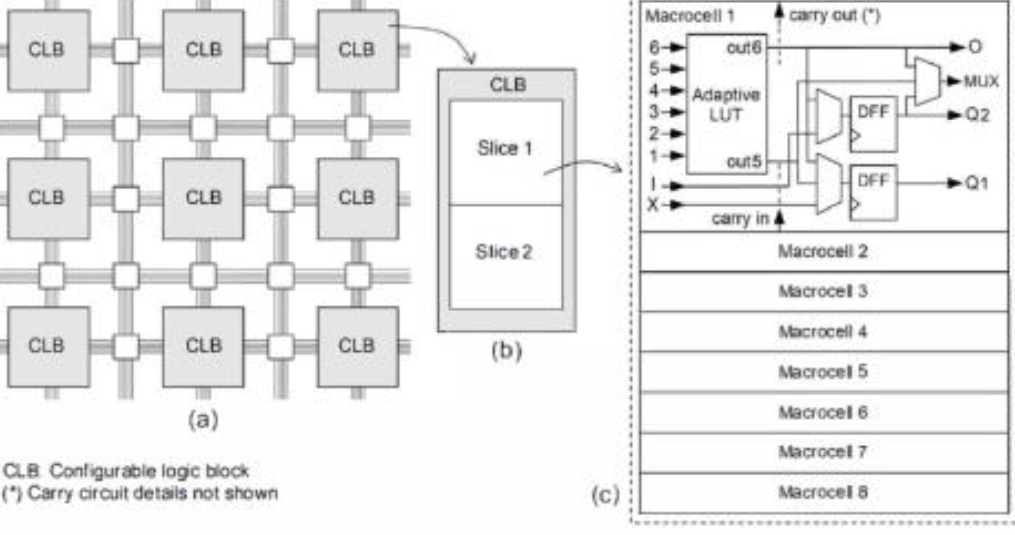
\includegraphics[width=0.75\textwidth]{FPGA Ultrascale+.png}
    \caption{Estrutura Interna da FPGA Ultrascale+}
    \label{fig:Ultrascale}
\end{figure}

Os sub-blocos das FPGAs são compostos por LUTs e registradores. As LUTs são compostas por uma árvore binária de multiplexadores 2:1, permitindo o armazenamento de uma função lógica na forma de SOP. Os registradores são os componentes síncronos dos sub-blocos. Além da estrutura mencionada, FPGAs comumente possuem diversos módulos integrados, como CPUs, DSPs, memória Flash, PLLs, que aumentam ainda mais as capacidades do FPGA.

As FPGAs são programadas utilizando uma linguagem de descrição de hardware, sendo o VHDL uma das mais comuns para a síntese de circuitos integrados de alta velocidade. Criada por uma iniciativa financiada pelo Departamento de Defesa dos Estados Unidos em meados dos anos 80, o VHDL foi a primeira linguagem de descrição de hardware padronizada pela IEEE.

A estrutura de um código VHDL consiste em três partes principais: declaração de bibliotecas/pacotes, entidade e arquitetura. Na primeira parte, são listadas as bibliotecas e pacotes necessários para o projeto. As bibliotecas padrão incluem a `std` e a `work`. A entidade, que é a interface do sistema, descreve as entradas e saídas e é dividida em duas partes: parâmetros e conexões. Os parâmetros são valores constantes, como a largura de um barramento, que são declarados como genéricos. As conexões, por sua vez, definem a transferência de informações e correspondem aos pinos de entrada e saída do circuito. Já a arquitetura é a parte principal do sistema, na qual o circuito é descrito. Nessa seção, são definidas as atribuições, operações lógicas e aritméticas, comparações, entre outros. Há também uma parte declarativa da sintaxe, que apresenta uma ampla variedade de declarações possíveis.

Dessa forma, circuitos digitais para processamento de sinais em tempo real são muito utilizados em sistemas de comunicações sem fio. Um exemplo de aplicação são os DPDs para transmissores sem fio. Os DPDs são baseados em operações matemáticas que envolvem uma grande quantidade de somas, produtos e tabelas de busca. Devido às rigorosas exigências de frequência de operação, torna-se fundamental a paralelização das operações necessárias. Nesse contexto, as FPGAs se mostram uma alternativa viável para a implementação de circuitos DPDs, especialmente devido à sua capacidade de paralelização. Considerando que a paralelização em FPGAs pode alcançar uma taxa de operação adequada para o uso pretendido, a implementação desse hardware em um circuito lógico dedicado pode oferecer resultados ainda mais eficientes para essa aplicação, dado o potencial de otimização específica e o desempenho superior de circuitos dedicados em relação a arquiteturas reconfiguráveis.

\section{Síntese com as células da tecnologia}
A concepção o circuito lógico do DPD segue o fluxo de projeto VLSI para design de um circuito integrado de aplicação específica, inclui a descrição do circuito em VHDL, síntese lógica utilizando as células padrão da tecnologia, PAR (\textit{place and route}) e simulações comportamentais e temporais. O diagrama do fluxo VLSI pode ser ilustrado pela figura \ref{fig:CMOS2010}.

\begin{figure}[ht!]
	\centering
	\captionsetup{justification=centering}
	\caption*{Fonte: \cite{CMOS2010}}
	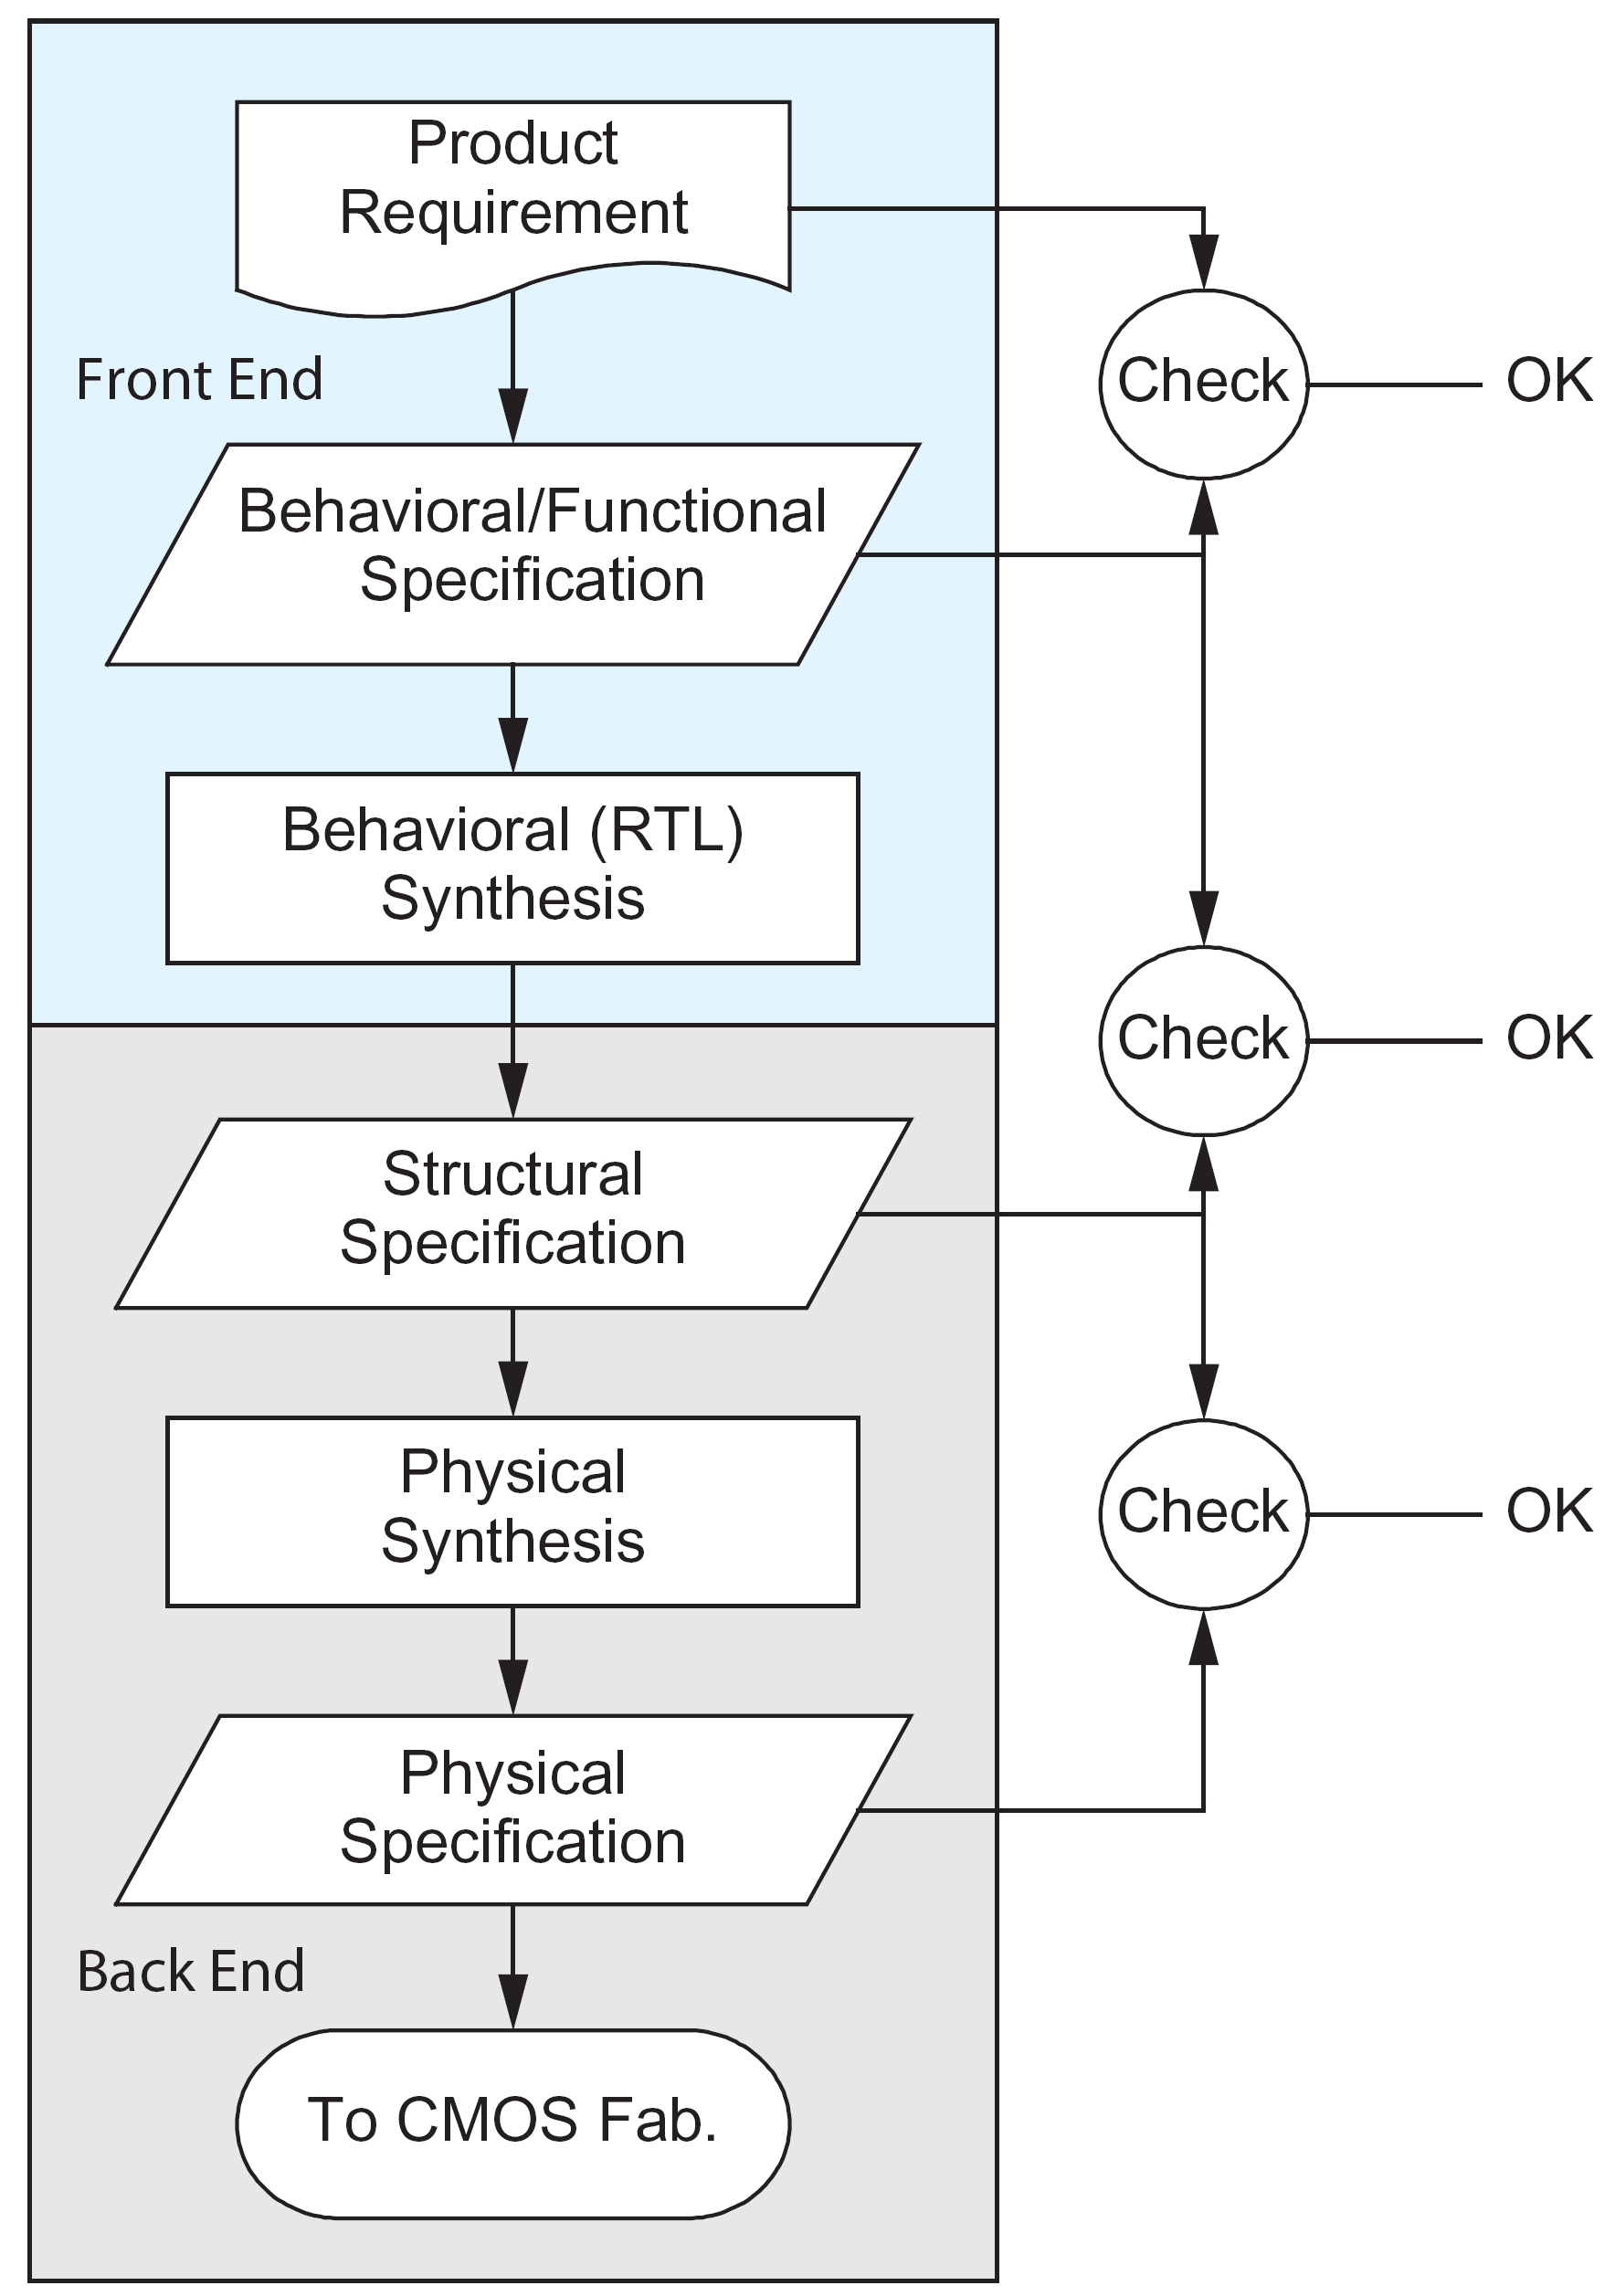
\includegraphics[width=0.25\textwidth]{fluxovlsi.png}
	\caption{Fluxo de projeto VLSI.}
	\label{fig:CMOS2010}
\end{figure}

No desenvolvimento do circuito, várias etapas são seguidas. Inicialmente, realiza-se a simulação comportamental para assegurar que o circuito descrito em VHDL cumpre os requisitos esperados, utilizando um \textit{testbench} em VHDL e a ferramenta Cadence NCLaunch. Posteriormente, ocorre a síntese lógica a partir do modelo comportamental, empregando a ferramenta Genus para gerar um modelo RTL com células padrão de uma tecnologia específica, levando em conta restrições de área, frequência e consumo de energia. Essa síntese resulta em dois arquivos: um em Verilog, contendo componentes e conexões, e outro com informações de atraso no formato SDF. A simulação pós-síntese é então executada para validar o netlist gerado, utilizando o mesmo \textit{testbench} da simulação comportamental. Na etapa de PAR, o layout é desenvolvido posicionando as células e estabelecendo as conexões entre elas, com o uso da ferramenta Innovus. Finalmente, na simulação pós-PAR, o circuito é avaliado considerando as resistências e capacitâncias parasitas. Cada etapa é crucial para assegurar o funcionamento correto do circuito.



\chapter{Material e Métodos} 
\label{chap:mati}
Como mencionado anteriormente, este trabalho tem como objetivo desenvolver o design de um circuito integrado para um DPD, partindo de um modelo previamente validado tanto em software quanto em hardware, especificamente em FPGA. O projeto foi dividido em quatro etapas principais:

\begin{itemize}
\item Estudo do DPD;
\item Implementação em software;
\item Implementação em FPGA;
\item Design e validação do circuito integrado.
\end{itemize}


\section{Estudo dos DPDs}
A etapa consistiu no estudo dos DPDs, conforme apresentado no Capítulo \ref{chap:revi}, onde foi feito todo o levantamento sobre os tipos de modelagem dos DPDs. O objetivo deste estudo é entender as diferentes abordagens de modelagem, avaliar seus desempenhos e identificar as mais adequadas para a aplicação em amplificadores de potência.

\section{Implementação em software} \label{sec:implsoft}

Nesta etapa, foi realizada a implementação do modelo DPD em software, utilizando a linguagem de programação Python. Esta linguagem amigável e amplamente difundida na comunidade acadêmica.

Para essa modelagem, foram coletados sinais de entrada e saída de um amplificador de potência classe AB, que utiliza um HEMT fabricado com tecnologia GaN. O amplificador foi excitado por um sinal portador de frequência de 900 MHz, modulado por um sinal de envelope WCDMA 3GPP com aproximadamente 3,84 MHz de largura de banda. Os dados de entrada e saída do amplificador de potência foram medidos usando um VSA Rohde \& Schwarz FSQ com uma taxa de amostragem de 61,44 MHz, conforme disponível em \cite{Bonfim2016}.

Em seguida, realizou-se o cálculo da estimativa do sinal utilizando números com vírgula fixa. Para verificar a precisão dessa estimativa em relação ao sinal original, calculou-se o NMSE. Para essa validação, os dados foram inicialmente divididos em conjuntos de extração e validação. A matriz de extração foi calculada com os dados de extração, utilizando o código disponível no anexo \ref{cod:mp}. Esse cálculo é essencial para a extração dos coeficientes do polinômio de memória. Após a extração dos coeficientes, calculou-se o modelo do PA, que foi então validado com os dados de validação. O NMSE obtido para um polinômio de 2° grau com uma amostra memorizada foi de -23,57 dB.

Em seguida, o algoritmo foi ajustado para operar com números em vírgula fixa e o número total de bits foi reajustado para atingir a menor resolução possível, buscando o menor NMSE simulado, conforme ilustrado pelo anexo \ref{cod:mpint}. Por ser tratar de um cálculo em virgula fixa, fez-se necessário uma readequação do resultado obtido entre cada multiplicação de forma a manter a resolução inicial.

\section{Implementação em FPGA}
Essa etapa consiste na implementação do DPD em FPGA. Para isso, é necessário realizar paralelizações nas operações aritméticas. A Figura \ref{fig:diagramaprocess} ilustra como esse processo está dividido entre cada ciclo de clock. Aqui está o trecho reescrito de forma mais clara: A cada ciclo, duas operações são realizadas em paralelo: o sinal atual é elevado ao quadrado e registrado, enquanto ocorre o somatório do produto entre os sinais do mesmo instante de tempo e seus respectivos coeficientes. Esse processo ocorre P vezes para os \( P \) graus do polinômio de memória. Portanto, a saída do DPD é incompleta para os primeiros \( P \) períodos de clock, pois, nesses primeiros ciclos, realiza-se o cálculo com base em entradas de sinais anteriores que ainda não ocorreram, resultando em uma saída incompleta.

\begin{figure}[ht!]
  \centering
  \captionsetup{justification=centering}
  \caption*{Fonte: Autor}
  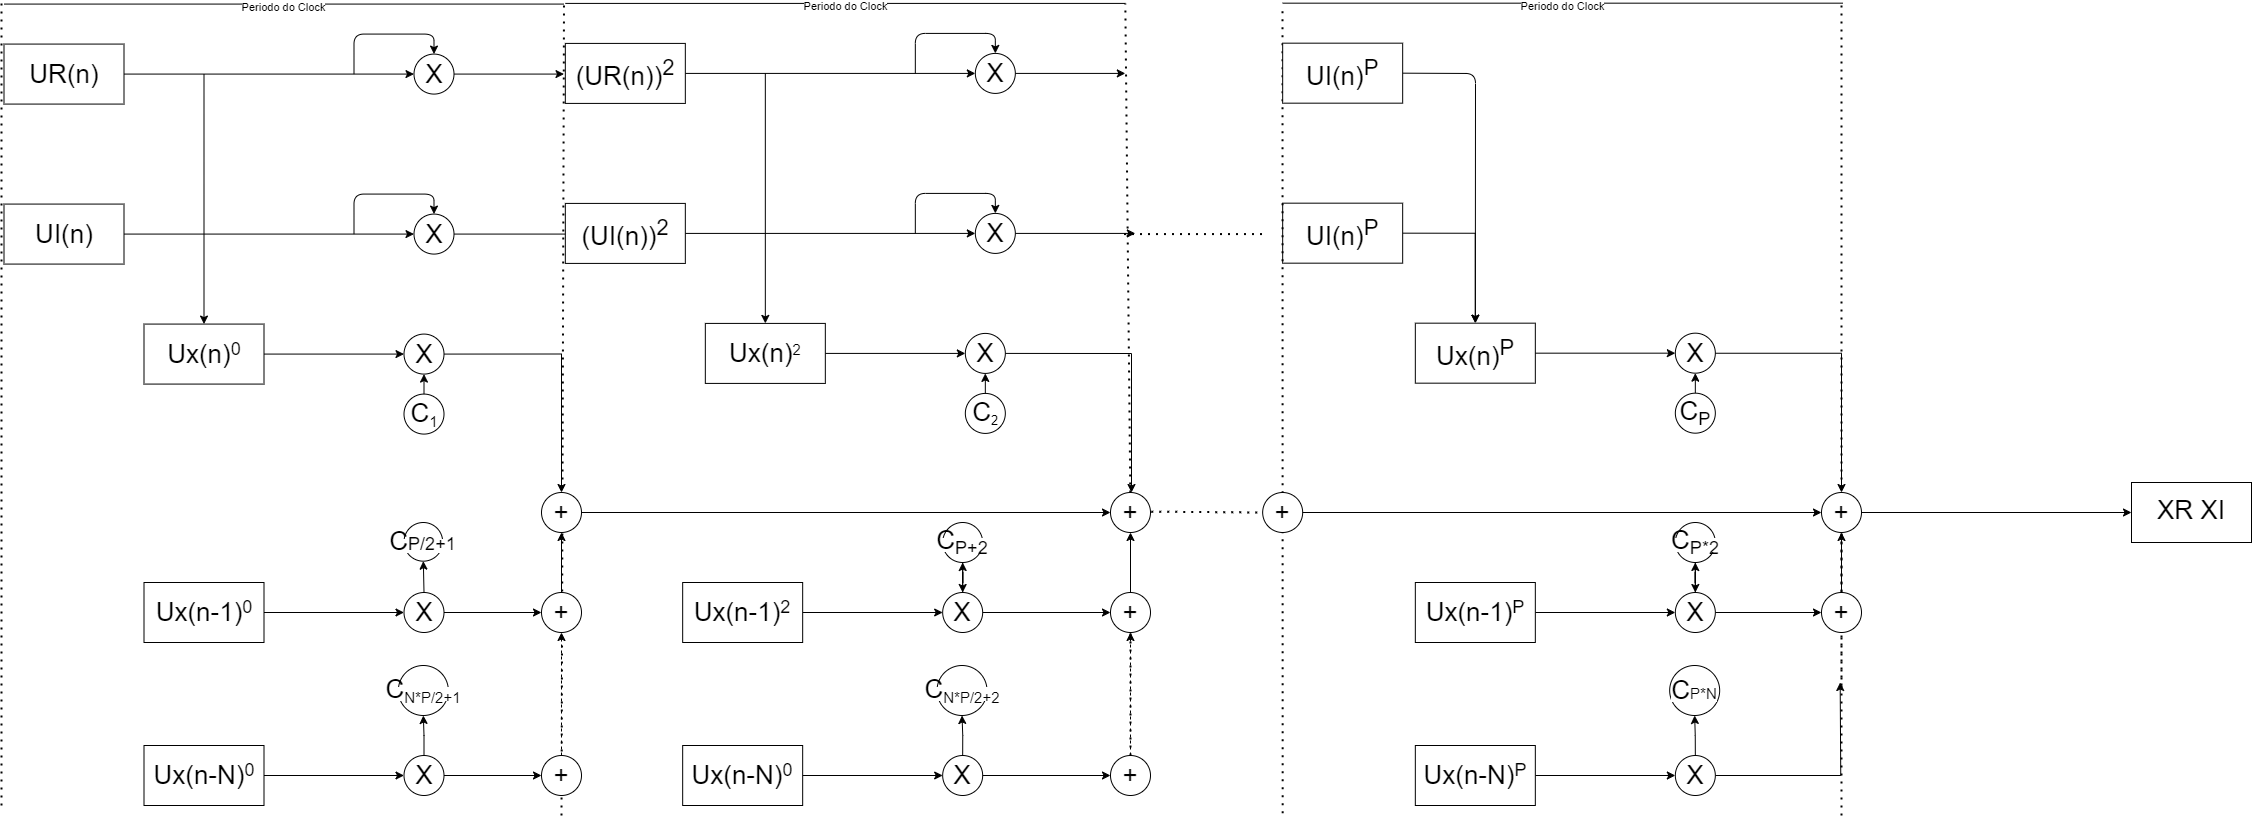
\includegraphics[width=0.80\textwidth]{diagrama_process.png}
  \caption{Processo de cálculo da saída}
  \label{fig:diagramaprocess}
\end{figure}

\section{Design e validação}
Finalmente, na última etapa, realiza-se o processo de concepção do circuito integrado do DPD como um circuito dedicado integrado na tecnologia BiCMOS 130 nm 8HP, utilizando as ferramentas específicas de desing de circuito integrado.
O fluxo de projeto VLSI para design de um circuito integrado de aplicação específica, inclui a descrição do circuito em VHDL, síntese lógica utilizando as células padrão da tecnologia, PAR (\textit{place and route}) e simulações comportamentais e temporais. O diagrama do fluxo VLSI pode ser ilustrado pela figura \ref{fig:CMOS2010}.

\begin{figure}[ht!]
  \centering
  \captionsetup{justification=centering}
  \caption*{Fonte: \cite{CMOS2010}}
  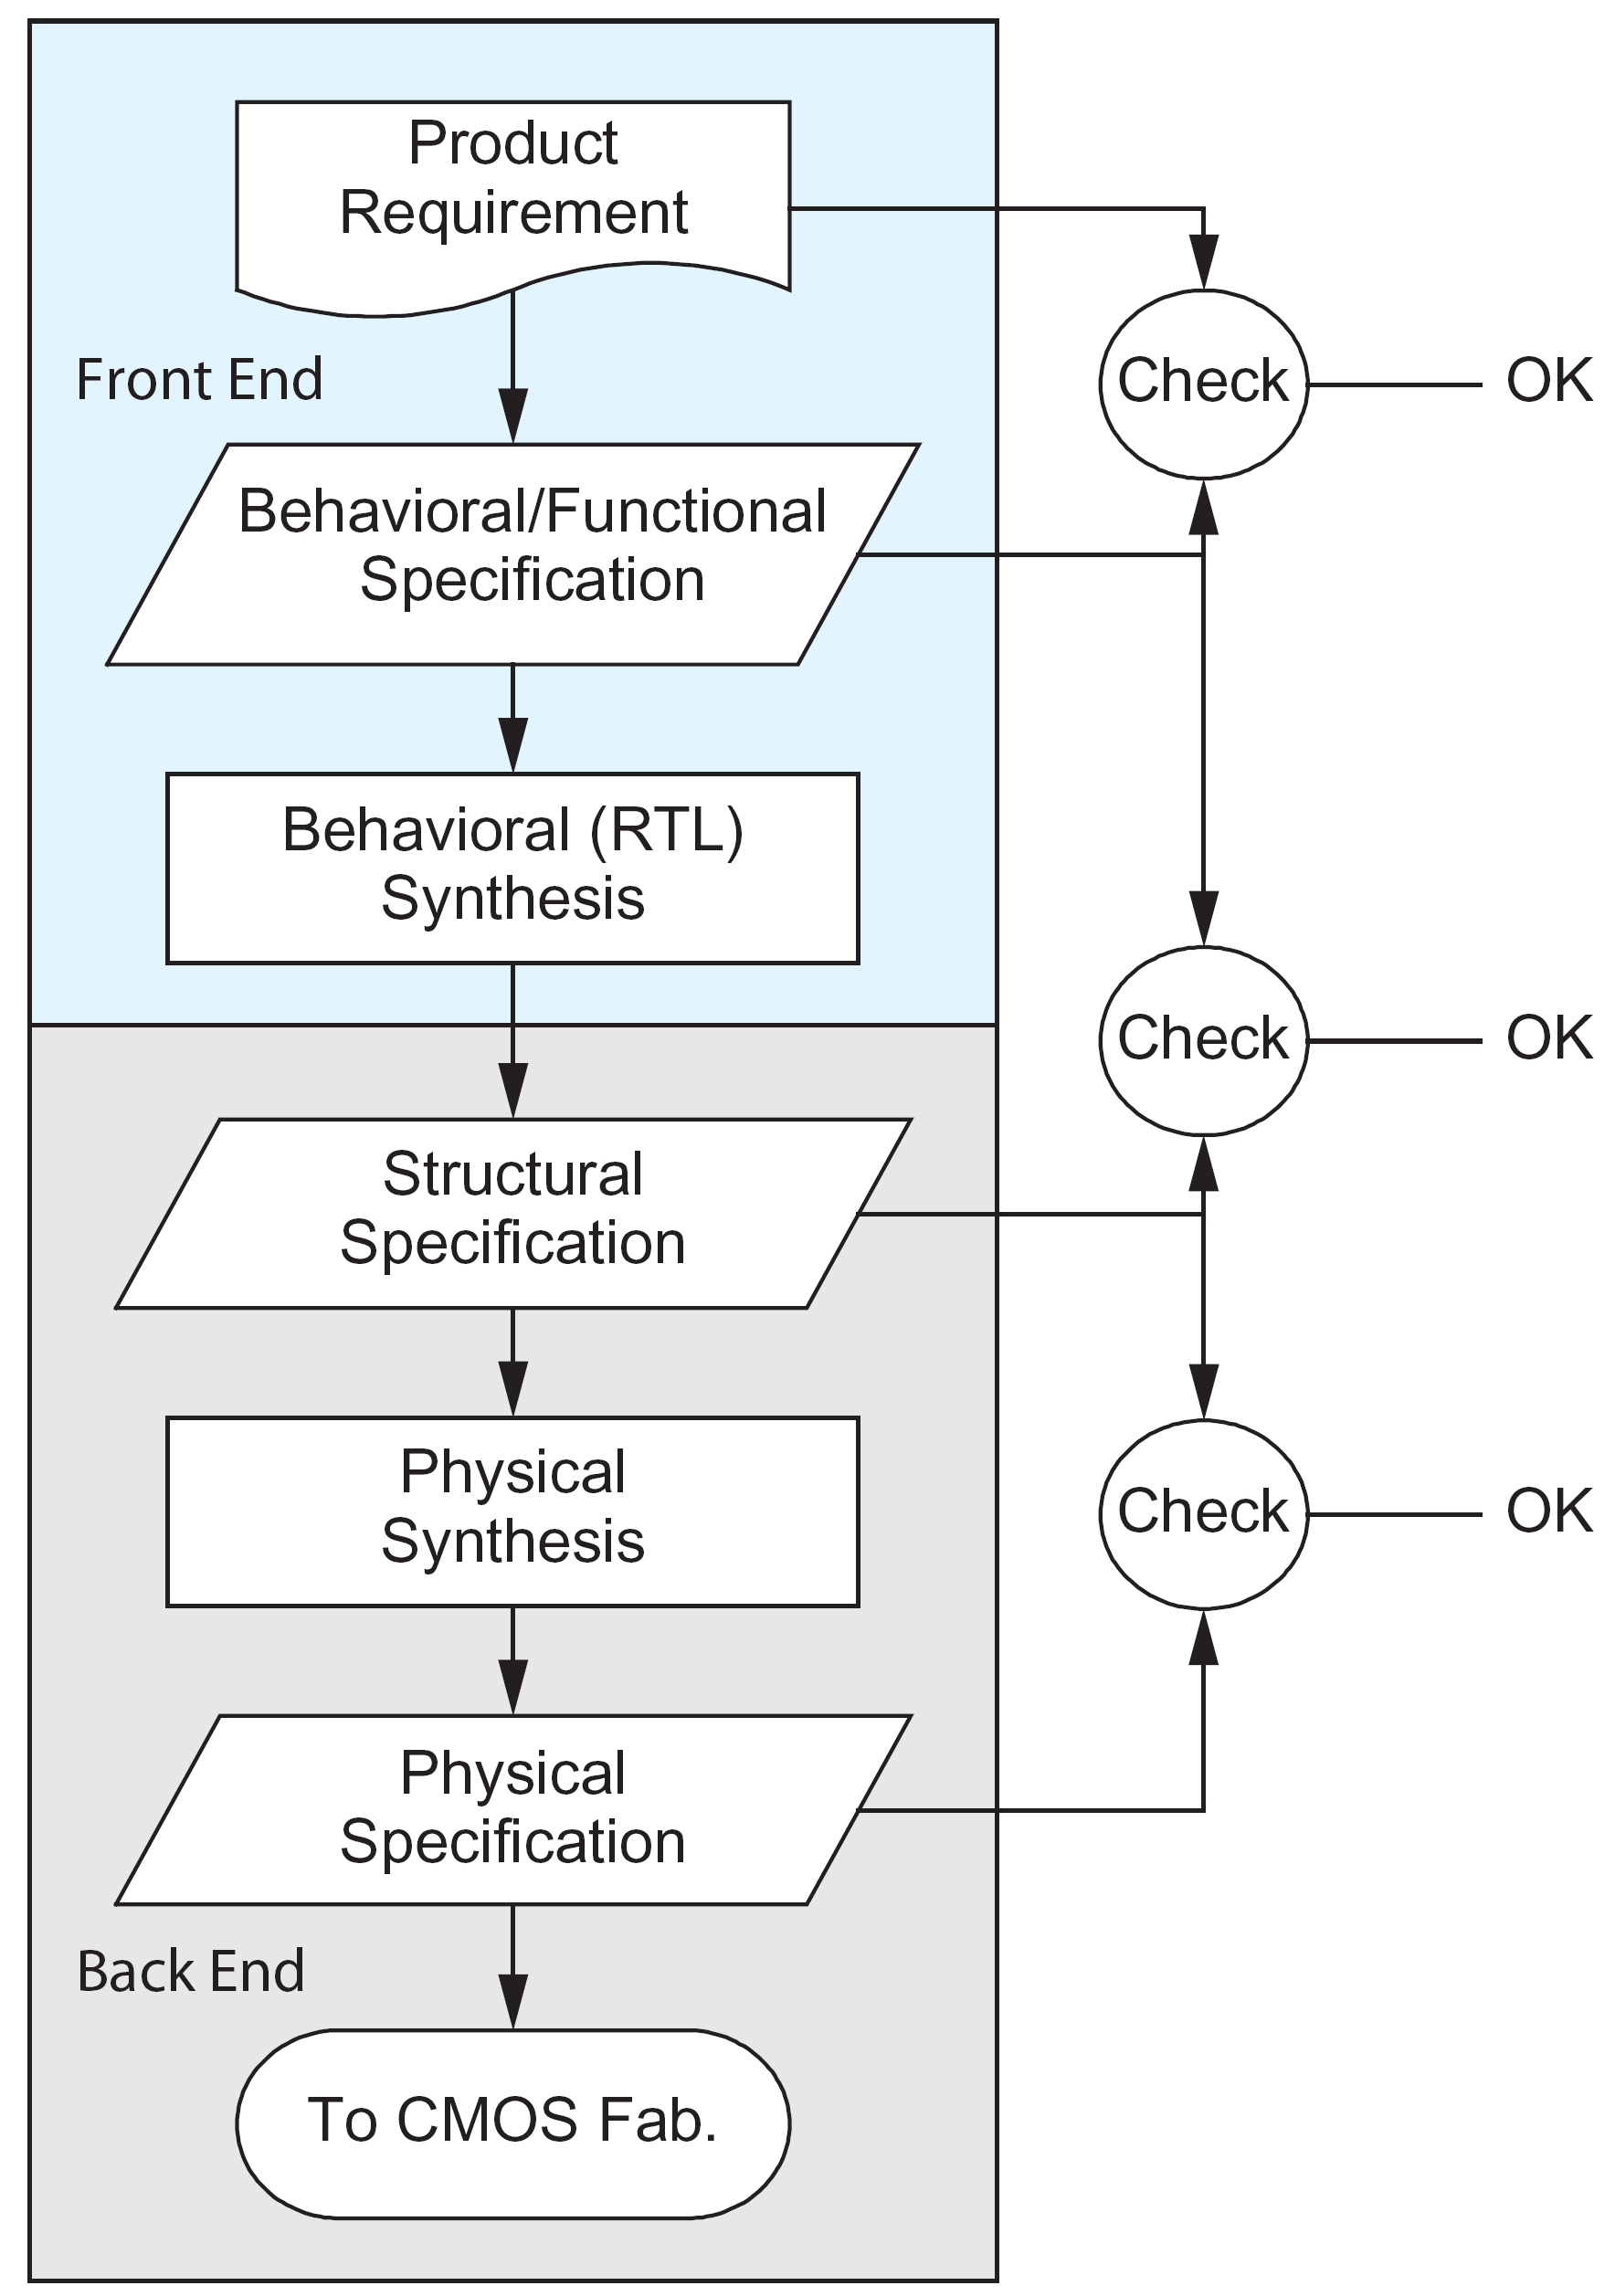
\includegraphics[width=0.25\textwidth]{fluxovlsi.png}
  \caption{Fluxo de projeto VLSI.}
  \label{fig:CMOS2010}
\end{figure}

No processo de desenvolvimento do circuito várias etapas são executadas. Primeiro, há a simulação comportamental para verificar se o circuito descrito em VHDL atende às expectativas, utilizando um \textit{testbench} em VHDL e a ferramenta Cadence NCLaunch. Em seguida, ocorre a síntese lógica, onde a partir do modelo comportamental, utiliza-se a ferramenta Genus para criar um modelo RTL com células padrão de tecnologia específica, considerando restrições de área, frequência e consumo de energia. A síntese gera dois arquivos: um com componentes e conexões, em Verilog, e outro com informações de atraso no formato SDF. A simulação pós-síntese é realizada para validar o netlist gerado usando o mesmo \textit{testbench} da simulação comportamental. Em seguida, na etapa de PAR, o layout é criado posicionando as células e realizando as conexões entre essas células, utilizando a ferramenta Innovus. Por fim, na simulação pós-PAR, o circuito é simulado considerando as resistências e capacitâncias parasitas. Cada etapa é fundamental para garantir o correto funcionamento do circuito.  

\chapter{Resultados e Discussão} 
\label{chap:resul}
\subsection{Modelagem do PA}

Para fazer a modelagem em software foi utilizada a linguagem de programação Python. Para isso, separou-se os dados citados na seção \ref{sec:implsoft}, em dados de extração e dados de validação, os quais são utilizados para extração dos coeficientes do modelo do MP e validação do modelo encontrado, respectivamente. Para fazer a validação do modelo utilizou-se a métrica do NMSE, que consiste em calcular o erro quadrático médio do valor medido pelo VSA (Analisador de Sinal Vetorial) para o valor calculado pelo modelo. Portanto, quanto menor o NMSE mais fiel é o modelo do PA. Nesta etapa obteve-se um NMSE de -23.57 dB, para cálculos em vírgula flutuante, onde o resultado está presente no gráfico da figura \ref{fig:modelopafloat}.

\begin{figure}[htbp]
    \centering
    \captionsetup{justification=centering}
    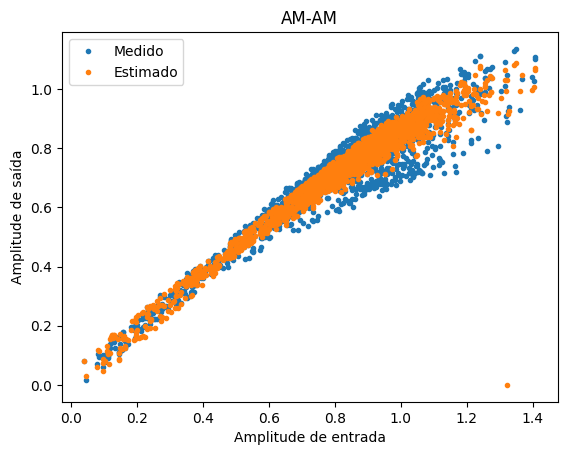
\includegraphics[width=\figsize]{modeloPAfloat.png}
    \caption{Modelo do PA em vírgula flutuante}
    \label{fig:modelopafloat}
\end{figure}

\subsection{Definição do número de bits}

Após concluída a modelagem matemática, realizou-se a modelagem do PA para então ser feito o levantamento da quantidade de bits necessários para a implementação do DPD em hardware minimizando os erros de quantização. 
Para isso foi necessário refazer a extração dos coeficientes, mas desta vez com os dados normalizados para valores de 0 a $2^{bits}$.  
O resultado desse levantamento está presente no gráfico na figura \ref{fig:bits}.

\begin{figure}[htbp]
    \centering
    \captionsetup{justification=centering}
    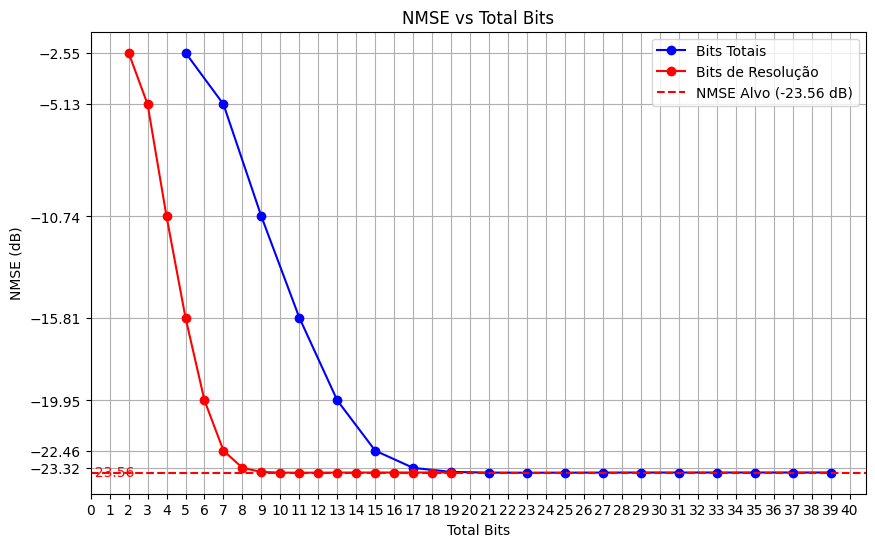
\includegraphics[width=\figsize]{bits.png}
    \caption{Gráfico Número de bits x NMSE}
    \label{fig:bits}
\end{figure}

Neste gráfico observa-se duas curvas, a curva em azul apresenta a quantidade total de bits contando com os bits de overflow necessárias para as operações de multiplicação, enquanto a curva em vermelho representa a quantidade de bits de resolução do sinal. Analisando este gráfico observou-se que não existem ganhos significativos no erro a partir de 8 bits, portanto foi feita a modelagem do PA utilizando uma resolução de 8 bits. O resultado alcançado está ilustrado pela figura \ref{fig:modelopa}.

\begin{figure}[htbp]
    \centering
    \captionsetup{justification=centering}
    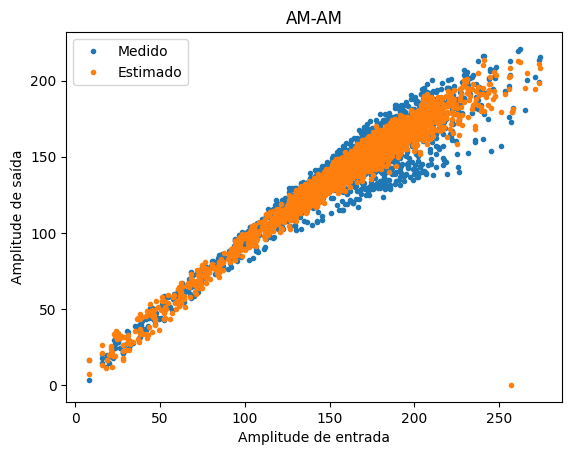
\includegraphics[width=\figsize]{modeloPA.png}
    \caption{Modelo do PA em vírgula fixa}
    \label{fig:modelopa}
\end{figure}

\subsection{Modelagem do DPD}
A partir dos resultados obtidos foi possível fazer a modelagem do DPD, para isso foi feito o mesmo processo de modelagem do PA, porém para alcançar a característica de transferência inversa do PA foi invertido a ordem dos dados de entrada e saída para extração dos coeficientes do DPD. O resultado desta modelagem está ilustrado pela figura \ref{fig:modelodpd} a seguir.

\begin{figure}[htbp]
    \centering
    \captionsetup{justification=centering}
    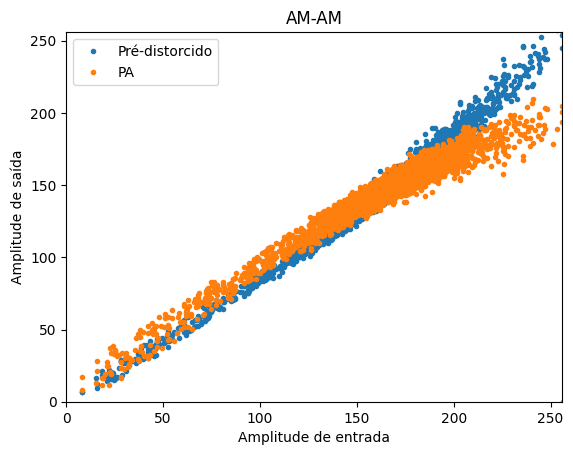
\includegraphics[width=\figsize]{modelodpd.png}
    \caption{Modelo do DPD em vírgula fixa}
    \label{fig:modelodpd}
\end{figure}

\subsection{Implementação do DPD em FPGA}

E por fim foi implementado o código em VHDL para FPGA.
Para que essa arquitetura de hardware apresentasse uma boa performance, todas as operações aritméticas (soma e multiplicação) são realizadas de forma síncrona. Então foi necessário dividir cada uma em processos distintos. A saída de um processo alimenta um \textit{buffer}, que serve como entrada para o próximo processo. A Figura \ref{fig:diagramaprocesssimpl} ilustra essa arquitetura de maneira simplificada.

\begin{figure}[htbp]
	\centering
	\captionsetup{justification=centering}
	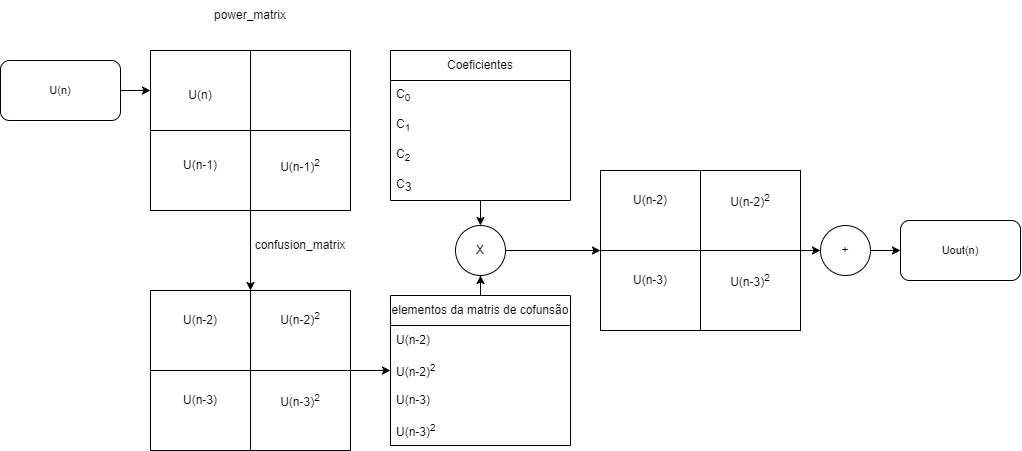
\includegraphics[width=\figsize]{fluxo_de_calculo.png}
	\caption{Processo de cálculo da saída}
	\label{fig:diagramaprocesssimpl}
\end{figure}

O resultado dessa implementação foi simulado em uma FPGA Virtex5 XC5VLX50T, utilizando um total de 150 registradores, 692 LUTs e 4 DSP48Es, operando a uma frequência de 61,44 MHz. A Figura \ref{fig:fpgasim} apresenta o resultado dessa implementação, representado pelos "x" em vermelho, em comparação com o resultado da simulação em Python, indicado pelos "." em azul.

\begin{figure}[htbp]
	\centering
	\captionsetup{justification=centering}
	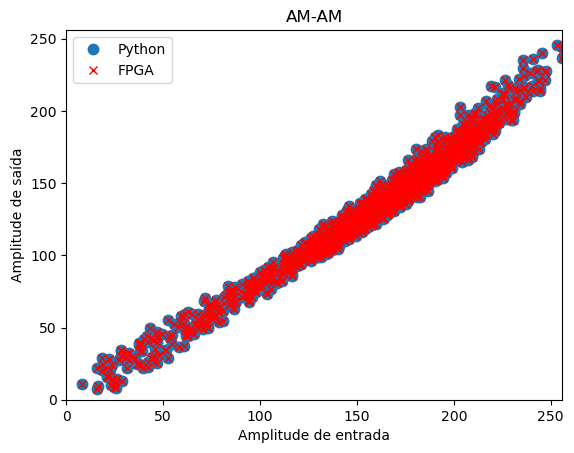
\includegraphics[width=\figsize]{fpgasim.png}
	\caption{Processo de cálculo da saída}
	\label{fig:fpgasim}
\end{figure}


\chapter{Conclusão} 
\label{chap:conc}
A evolução dos sistemas de comunicação sem fio tem promovido a implementação de diversos serviços móveis, tornando essencial que esses sistemas operem com máxima eficiência. Nesse cenário, a implementação de um DPD em cascata com o PA surge como uma alternativa de baixo custo e interessante para melhorar o desempenho desses sistemas.
O objetivo deste trabalho de conclusão de curso é implementar em hardware um DPD baseado no modelo de Polinômio de Memória. Para isso, o projeto foi dividido em quatro etapas: estudo do DPD e da modelagem matemática, modelagem do DPD em software, implementação do DPD em hardware e, finalmente, design do circuito integrado.
Sendo assim a primeira etapa de desenvolvimento do projeto foi a modelagem do PA em virgula flutuante, utilizando o método do MP, para fazer essa modelagem utilizou-se um polinômio de 2° grau com uma amostra de memória, para fazer a validação dessa modelagem uitlizou-se a métrica do NMSE. Nesta etapa obteve-se um NMSE de -23,57 dB, a próxima etapa consiste em otimizar a quantidade de células lógicas utilizadas no processo limitando o número de bits utilizados. Nesta etapa observou-se que a partir de 8 bits, não havia melhora expressiva no NMSE, assim, essa foi a resolução em bits utilizadas para a amostragem de sinais. E por fim foi feito a modelagem do DPD em software o qual apresentou um comportamento inverso em relação o do PA, assim satisfazendo as necessidades.  Atualmente, o projeto está na etapa 3, que corresponde à implementação em hardware.  
Conclui-se, portanto, que o projeto alcançou os resultados esperados, com uma modelagem eficaz do PA e do DPD, satisfazendo os critérios de desempenho estabelecidos nas etapas iniciais.

% ----------------------------------------------------------
% Referências bibliográficas
% ----------------------------------------------------------

%\setlength{\afterchapskip}{\baselineskip}

\bibliography{Referencias}

% ----------------------------------------------------------
% ELEMENTOS PÓS-TEXTUAIS
% ----------------------------------------------------------
\postextual
% ----------------------------------------------------------

% ----------------------------------------------------------
% ANEXOS
% ----------------------------------------------------------

% \begin{apendicesenv}

% \partapendices

% \chapter*{\normalsize APÊNDICE A - Digite o cabeçalho do apêndice}

Apêndice: texto ou documento elaborado pelo autor, a fim de complementar sua argumentação, sem prejuízo da unidade nuclear do trabalho.

\chapter*{\normalsize APÊNDICE B - Digite o cabeçalho do apêndice}

% \end{apendicesenv}

\begin{anexosenv}

\partanexos
%\addcontentsline{toc}{chapter}{\hspace{2.105cm}ANEXOS}
\renewcommand{\ABNTEXchapterfontsize}{\ABNTEXsectionfont}

\section{\normalsize ANEXO A - função que calcula matriz de confusão em vírgula flutuante}
\label{cod:mp}
\small % Altera o tamanho da fonte
\begin{lstlisting}[language = Python, ]
def mp(P, M, xn):
    L = xn.shape
    XX = np.zeros((L[0] - M, P * (M+1)), dtype=np.complex128)
    for l in range(M+1, L[0]):
        for p in range(1, P+1):
            for m in range(0, M+1):
                XX[l-M-1, ((p-1)*(M+1))+m] = (np.abs(xn[l-m])**(2*p-2)*(xn[l-m]))[0]
    return XX

XX_ext = mp(P, M, in_data_ext)
coefficients, _, _, _ = np.linalg.lstsq(XX_ext, out_data_ext[M:], rcond=None)
predicted_val = XX_val @ coefficients

\end{lstlisting}

\section*{\normalsize ANEXO B - Função que calcula matriz de confusão em vírgula fixa}

readeq = lambda val, precision: np.floor(val / (2 ** precision))

\label{cod:mpint}
\small % Altera o tamanho da fonte
\begin{lstlisting}[language = Python, ]
    def mp_int(P, M, xn, bits):
    L = xn.shape
    XX = np.zeros((L[0] - M, P * (M+1)), dtype=np.complex128)
    for l in range(M+1, L[0]):
        for p in range(1, P+1):
            for m in range(0, M+1):
                    A = np.real(xn[l-m])[0]
                    B = np.imag(xn[l-m])[0]
                    modulo_power = 2**bits 
                    modulo_square = readeq(A ** 2 + B ** 2, bits)
                    for _ in range(1, p):
                       modulo_power = readeq(modulo_power * modulo_square, bits)
                    real_part = readeq(A * modulo_power,bits)
                    imag_part = readeq(B * modulo_power,bits)
                    XX[l-M-1, ((p-1)*(M+1))+m] = complex(real_part,imag_part)        
    return XX

\end{lstlisting}


\end{anexosenv}


\end{document}